%\part{Fundamentação Teórica}
\chapter{\textit{Radio Frequency Identification} (RFID)}


Identificação por radio frequência (RFID) é uma tecnologia de identificação automatizada que utiliza etiquetas (\textit{tags}) para transmitir dados para leitores de RFID \cite{li2009} . Esta tecnologia possui diversas aplicações, sendo utilizada amplamente no mercado em cartões de identificação pessoal, identificação e controle de animais e processos migratórios, rastreamento de mercadorias em cadeias de fornecimento e aplicações gerais de monitoramento e identificação. Seu baixo custo de implementação e múltiplas utilidades fazem com que essa tecnologia venha crescendo de forma exponencial em diversos setores da sociedade. 

A tecnologia RFID utiliza a radiofrequência para obter dados de uma \textit{tag} de forma remota, sem a necessidade de ligações físicas e sem apresentar limitações para atravessar obstáculos como paredes ou encapsulamentos. 
A \textit{tag} é fixada no objeto a ser monitorado e possui em sua memória os dados básicos sobre o objeto, como números de série. Esses dados são então recebidos pelo leitor quando a \textit{tag}  entra em seu campo magnético. Por fim, os dados são processados por uma central para que possa ser feita a identificação ou outras ações pertinentes. O diagrama da Figura \ref{rfid-geral} mostra o funcionamento geral do sistema completo.

\begin{figure}[h!]
  \centering
  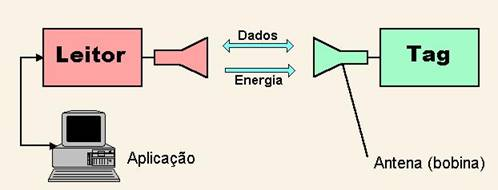
\includegraphics[width=0.5\textwidth]{figuras/image002.jpg}
  \caption{Funcionamento geral do sistema RFID.\cite{Sangreman}}
  \label{rfid-geral}
\end{figure}

A comunicação entre o leitor e a \textit{tag} é controlada por protocolos, como por exemplo o ISO/IEC 14443, ISO/IEC 18001, etc. A escolha do protocolo depende de diversos fatores como frequência de operação, aplicação e o número de \textit{tags} a serem identificadas. Os diversos protocolos existentes e suas particularidades serão abordados mais à frente.

%\newpage

\section{Arquitetura de uma \textit{Tag} de RFID}

A \textit{tag} é o componente fixado no objeto a ser monitorado e carrega todas as informações básicas que possam ser de interesse para o monitoramento, podendo ser uma \textit{tag} apenas de leitura ou de leitura e escrita, dependendo da aplicação.

Este componente é a parte principal do sistema RFID e consiste basicamente em um \textit{chip} e uma antena. O \textit{chip} possui o bloco analógico e de RF, memória e um bloco de controle. Dependendo do tipo de tecnologia (ativa, semi-ativa ou passiva) e da frequência de operação, sua arquitetura para armazenamento de dados, comunicação e fonte de energia podem diferir. \cite{markham}

No caso das \textit{tags} passivas, sua fonte de alimentação é a própria onda eletromagnética incidente, não sendo necessária uma fonte de alimentação externa para a mesma. A \textit{tag} absorve a energia da onda eletromagnética que carrega as informações enviadas pelo  leitor.

O circuito da \textit{tag} é formado por dois grandes blocos (controle digital e o bloco de \textit{front-end} analógico) e uma memória (Figura \ref{11}). O circuito de \textit{front-end} analógico, por sua vez, é formado pelos seguintes blocos\cite{jose}:

\begin{itemize}

\item Retificador: bloco que retifica o sinal de RF de entrada e gera a tensão DC necessária para alimentar os outros blocos do sistema;
\item Demodulador: Bloco receptor do sistema que detecta os comandos enviados pelo leitor. Também extrai o clock a partir do sinal RF recebido, que é necessário para sincronizar o RFID com o leitor. 
\item Modulador: Bloco transmissor do sistema que envia à \textit{tag} o ID de identificação para o leitor RFID. 
\item Clock interno: Gerador de clock interno que fornece um clock gerado para a parte digital do circuito. 

\end{itemize}


\section{Frequências de funcionamento do sistema de RFID}

Para a padronização do uso das \textit{tags}, as normas técnicas disponíveis determinam os intervalos de frequência em que a \textit{tag} deve funcionar para determinadas aplicações:

\begin{itemize}

\item \textit{Low Frequency}: De 30 kHz até 300 kHz. As etiquetas desta faixa de frequências operam em 125 kHz ou 134,2 kHz. Geralmente, são etiquetas passivas e seu maior uso é na identificação de animais, na forma de brincos ou implantes subcutâneos, e de pessoas também na forma de implantes subcutâneos. Distância de leitura é de alguns centímetros;

\item \textit{High Frequency}:  De 3 MHz até 30 MHz. Etiquetas construídas em 13,56 MHz, normalmente utilizadas como crachás para identificação individual ou então como meio de pagamento, por exemplo para o transporte público, tal como os bilhetes únicos. Também pode ser utilizado para identificar objetos individuais, como nas lojas de departamento em sistemas antifurto. A distância de leitura chega a ser maior do que 10 cm;

\item \textit{Ultra High Frequency}: De 300 MHz até 1 GHz. Nesta faixa, as \textit{tags} são fabricadas nas faixas de frequências de 433 MHz, para uso em rastreamento de cargas, tais como contêineres, vagões, caminhões e etc. Nessa faixa de frequências, as \textit{ tags} são ativas, ou seja, energizadas com baterias, e robustas. Outra faixa bastante utilizada é a de 868 MHz na Europa e de 915 MHz nos Estados Unidos e Brasil. Essas etiquetas também são empregadas em processos de rastreamento de ativos ou produtos em lojas, controle de estoque, inventários e identificação veicular, como por exemplo em pedágios eletrônicos;

\item Microondas: Acima de 1 GHz. Duas frequências para RFID: 2,45 GHz e 5,8 GHz. Esta faixa de frequências é utilizada em aplicações industriais, científicas e médicas. No Brasil, a principal aplicação de \textit{tags} nessa faixa de frequências é a de identificação veicular para o pedágio eletrônico. \cite{Puhlmann}

\end{itemize}


%\newpage

\section{Protocolos de comunicação entre o Leitor e a \textit{Tag}}

A criação de padrões de comunicação entre o leitor e a \textit{tag} é de extrema importância para que a tecnologia de RFID possa se consolidar no dia a dia da sociedade. Tais padrões asseguram que diferentes sistemas possam atuar em conjunto, eliminando problemas de compatibilidade e aumentando a segurança de ditos sistemas.

O desenvolvimento de padrões é de responsabilidade do comitê técnico de diferentes institutos de padronização. A ISO é uma união mundial de institutos de padronização e contribui com numerosos comitês e grupos de trabalho para o desenvolvimento de padrões para RFID\cite{Fink}.

 A Tabela \ref{tab1} descreve as particularidades de alguns padrões.

\begin{table}[h!]

\begin{tabular}{|l|l|}

\hline
\textbf{ISO standard} & \textbf{ Descrição}\\
\hline
ISO 11784 & RFID para animais - Estrutura de codigo\\
\hline
ISO 11785 & RFID para animais - Concepção técnica\\
\hline
ISO/IEC 14443A,B & Cartões de identificação - Cartões de proximidade\\
\hline
ISO/IEC 18001, 15961, 15962, 15963 & Gerenciamentos de diversos itens de RFID\\
\hline
ISO/IEC 18000-1 à 18000-4 & Comunicação por ar para diversas frequências\\
\hline

\end{tabular}
\caption{Descrições de ISOS para RFID \cite{markham}}\label{tab1}
\end{table}

%\subsection{Protocolo ISO/IEC 14443}

ISO/IEC 14443 é um padrão internacional de quatro partes para cartões inteligentes sem contato operando à 13.56 MHz em proximidade do leitor e será utilizado neste trabalho.

Tais cartões destinam-se a operar a aproximadamente 10 cm da antena do leitor. Cada parte do padrão é responsável por certas características do cartão:

\begin{itemize}

\item Parte 1 [ISO/IEC 14443-1:2000(E)]: define o tamanho e as características físicas do cartão. Lista também as condições ambientais que o cartão deve ser capaz de suportar sem danos permanentes às suas funcionalidades.

\item Parte 2 [ISO/IEC 14443-2:2001(E)]: define a potência de RF e a interface do sinal. São definidos na parte 2, dois esquemas de sinais, tipo A e tipo B. Ambos esquemas são \textit{half-duplex} com 106 kbit por segundo de taxa de dados em cada direção. Os dados transmitidos pelo cartão são modulados com um \textit{subcarrier} de 847.5 KHz. O cartão é alimentado pelo campo RF e não é dependente de baterias.

\item Parte 3 [ISO/IEC 14443-3:2001(E)]: define os protocolos de inicialização e anticolisão para os cartões tipo A e B. Os comandos, respostas, \textit{frame} de dados e o tempo do sistema de anticolisão serão definidos posteriormente. O esquema de inicialização e anticolisão é projetado para permitir a a construção de leitores de múltiplo protocolo capazes de se comunicar com placas de ambos tipos A e B.

\item Parte 4 [ISO/IEC 14443-4:2001(E)]: define os protocolos de transmissão de alto nível para cartões de tipo A e B. Os protocolos citados são opcionais para o padrão ISO/IEC 14443, ou seja, os cartões de proximidade podem ser projetados com ou sem os protocolos.\cite{14443} 

\end{itemize}

\newpage

\section{ASK - Amplitude Shift Key}

\textit{Amplitude Shift Keying}, no contexto de comunicações digitais, é um processo de modulação que atribui à uma senóide dois ou mais níveis discretos de amplitude. \cite{uri}

O sinal então modulado terá um valor zero para níveis lógicos baixos e o valor da saída do \textit{carrier} para níveis lógicos altos. A imagem \ref{ask} mostra um exemplo de sinal de entrada e a onda modulada em ASK.

\begin{figure}[ht!]
  \centering
  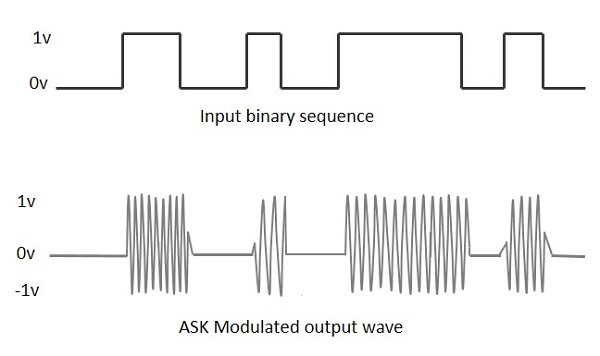
\includegraphics[width=0.8\textwidth]{figuras/ask.jpg}
  \caption{Exemplo de Sinal Modelado em ASK.}
  \label{ask}
\end{figure}


\chapter{Projeto de Circuitos Integrados Digitais}

Neste tópico, serão abordados os passos para o desenvolvimento de um projeto de circuitos integrados digitais, iniciando-se com a definição das especificações do projeto e validação de sua funcionalidade, e em seguida realizando-se as sínteses lógicas e físicas, finalizando o projeto com a verificação do layout obtido.

\section{Especificação e Validação da Funcionalidade}

Inicialmente, as áreas de interesse do projeto são identificadas para então se desenvolver planos de verificação \cite{Marlon}. As especificações devem ser totalmente respeitadas ao se modelar os blocos do sistema, ou seja, os formatos de dados, frequências de operação e todas as outras características de um bloco devem ser compatíveis com os demais blocos do sistema.

É neste ponto que as especificações determinadas por protocolos de comunicação são inseridas no sistema. Se essas regras forem seguidas, serão evitados problemas que poderiam atrasar o andamento do projeto  \cite{Marlon}. Assim, ao se obter a descrição em alto nível do sistema, o mesmo pode ser validado por meio de simulações mistas em ambientes como o MatLab/Simulink ou em linguagens como C/C++, SystemC e SystemC-AMS.

\section{Projeto RTL}

Com as especificações definidas e a funcionalidade validada, o próximo passo é o projeto RTL. Nesta etapa, são usadas linguagens de descrição de \textit{hardware} como o Verilog, SystemVerilog ou o VHDL para implementar os modelos funcionais obtidos na etapa anterior, utilizando-se componentes básicos como somadores e máquinas de estados.

É fundamental nesta etapa que os blocos funcionem sem nenhum erro e sigam à risca todas as especificações do projeto. Se estes blocos básicos não funcionarem como o requerido, todo o projeto pode apresentar falhas no fim. Por este motivo, as simulações de comportamento de cada bloco devem ser feitas e minuciosamente avaliadas.

\section{Simulação Funcional}

Para validar o funcionamento de cada bloco básico individual, é necessário realizar simulações comportamentais dos mesmos, analisando os sinais de saída de acordo com diferentes sinais de entrada usados para testes.

É feita a analise de cada bloco básico individual, bem como dos blocos maiores que são formados a partir destes. No fim, o bloco de mais alto nível (também chamado de \textit{top-level}) também deve ser simulado para que sua funcionalidade seja validada.

Essas simulações funcionais são feitas a partir de \textit{testbenches}, que são códigos nos quais são adicionados sinais de entrada de teste e outros sinais pertinentes ao bloco para permitirem a análise dos sinais de saída. A figura \ref{testb} mostra um exemplo de \textit{testbench } em Verilog.

\begin{figure}[h!]
  \centering
  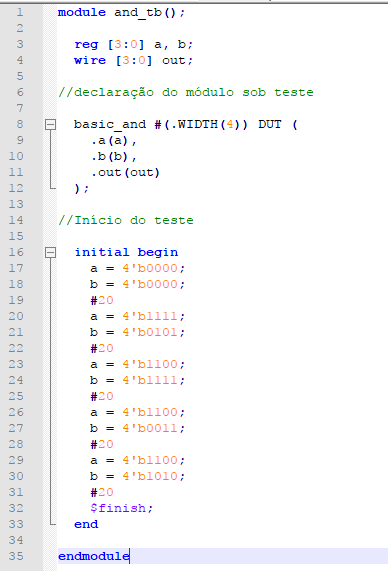
\includegraphics[width=0.5\textwidth]{figuras/test.PNG}
  \caption{\textit{Testbench} em Verilog.}
  \label{testb}
\end{figure}

É possível visualizar graficamente o comportamento dos sinais de entrada e de saída do módulo, como mostra a figura \ref{tests}, em ferramentas como o NCSim, da \textit{Cadence Design Systems}.

\begin{figure}[ht!]
  \centering
  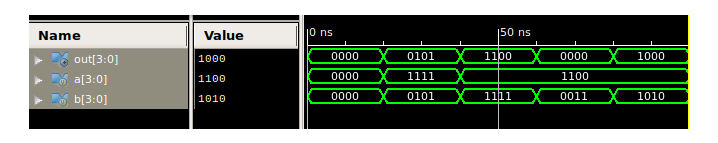
\includegraphics[width=\textwidth]{figuras/testsig.PNG}
  \caption{Visualização dos sinais de entrada e saída.}
  \label{tests}
\end{figure}

\section{Síntese Lógica}

Nesta etapa, o circuito comportamental que foi obtido na etapa anterior(em RTL) é sintetizado em termos de portas lógicas da biblioteca do fabricante, de acordo com a tecnologia na qual será implementado. Para esta tarefa são utilizadas ferramentas de síntese, como por exemplo a \textit{Design Compiler} da \textit{Synopsys}, a \textit{Genus Synthesis Solution} da \textit{Cadence Design Systems} e o \textit{Vivado} da \textit{Xilinx}, sendo esta última sendo voltada para FPGA's.

\section{Síntese Física}

A síntese física se inicia com a \textit{netlist} gerada pela síntese lógica. Essa \textit{netlist} descreve as conexões lógicas entre os componentes físicos como portas lógicas, I/O \textit{pins} e macro/IP \textit{blocks}. A síntese física então gera uma nova \textit{netlist} otimizada e um \textit{layout} equivalente. Seu objetivo é de satisfazer uma combinação de tempo, área, energia e roteabilidade.\cite{phy}

\section{Verificação de\textit{ Layout}}

A última etapa do projeto consiste em verificar a funcionalidade do \textit{layout} obtido.  Utilizando ferramentas computacionais, é necessário se certificar que a performance, tamanho, densidade e outros fatores estão dentro dos especificados na etapa inicial do projeto. Com um \textit{layout} seguindo as especificações e não apresentando problemas elétricos ou de outra natureza, o \textit{chip} está pronto para a fabricação.